\documentclass[12pt,oneside]{memoir} 

\usepackage[latinica, biblatex]{matfmaster} 
\usepackage{listings}
\usepackage{listings-golang}
\usepackage{color}
\usepackage{tikz}
\usepackage{pgfplots}
\usepackage{diagbox}
\usepackage{array}

\definecolor{background}{RGB}{255, 248, 220}


\lstset{ 
    frame=single,
    basicstyle=\footnotesize,
    keywordstyle=\color{blue},
    showstringspaces=false, 
    stringstyle=\color{red},
    tabsize=4,
    language=Golang
}

\lstnewenvironment{snippet}[1][]
    {\lstset{float=htpb,#1}} 
    {}



\bib{literatura}


\autor{Miloš Mitrović}
\naslov{Konkurentno programiranje u programskom jeziku Go}
\godina{2017}
\mentor{dr Milena \textsc{Vujošević Janičić}\\ Univerzitet u Beogradu, Matematički fakultet}
\komisijaA{dr Ana \textsc{Anić}\\  Univerzitet u Beogradu, Matematički fakultet}
\komisijaB{dr Laza \textsc{Lazić}\\  Univerzitet u Beogradu, Matematički fakultet}


\apstr{
text
}

\kljucnereci{programski jezik Go, konkurentno programiranje}

\begin{document}

\frontmatter
\naslovna
\komisija
\posveta{Mojoj sestri Ivoni}
\apstrakt
\tableofcontents*

\mainmatter

\chapter{Uvod}

% GO OPIS==============================================================================

\chapter{Karakteristike programskog jezika Go}

Go je imperativni programski jezik otvorenog koda koji razvija kompanija Google od 2007. godine. Napravljen je kao kompilirani jezik opšte namene sa statičkim tipovima koji podseća na interpretirane jezike sa dinamičkim tipovima. Podržava konkurentno programiranje, automatsko upravljanje memorijom kao i refleksiju tokom izvršavanja programa. Pogodan je za rešavanje svih vrsta problema a najviše se koristi za izgradnju servera, skriptove i samostalne aplikacije za komandnu liniju a može se korititi i za grafičke i mobilne aplikacije.

\section{Tipovi podataka}

Go je statički tipiziran jezik što znači da se varijabli dodeljuje tip prilikom njene deklaracije i on se ne može menjati tokom izvršavanja programa.  Za razliku od C-a Go ne podržava automatsku konverziju tipova već se konverzija mora navesti eksplicitno, u suprotnom se prijavljuje greška.\\

Od osnovnih ugrađenih tipova podataka Go podržava:
\begin{itemize}

\item Numeričke -  celobrojne označene (\texttt{int8}, \texttt{int16}, \texttt{int32}, \texttt{int64})
 i neoznačene  (\texttt{uint8}, \texttt{uint16}, \texttt{uint32}, \texttt{uint64}), u pokretnom zarezu (\texttt{float32}, \texttt{float64}) i kompleksne (\texttt{complex64}, \texttt{complex128})

\item Bulovske  (\texttt{bool})

\item Tekstualne (\texttt{string})

\end{itemize}

Od drugih vrsta podataka, Go podržava nizove, mape i slajseve - nizove sa promenljivom dužinom. Postoje i paketi koji omogućavaju rad sa listama.

\section{Funkcije i metodi}
 
\section{Interfejsi}

\section{Refleksija}

\section{Testiranje}

\section{Paketi}


% KONKURENTNO==============================================================================
\chapter{Konkurentno programiranje u programskom jeziku Go}

\section{Osnovni pojmovi konkurentnog programiranja}

\section{Mogućnosti u Go-u}

\subsection{Go-rutine}

\subsection{Kanali}

\subsection{Sinhronizacija}

\subsection{"Data race" detektor}

\begin{figure}
\begin{center}

\begin{verbatim}
WARNING: DATA RACE
Write at 0x00c420072006 by goroutine 18:
  main.mark_prime()
      /home/cg/root/7238354/main.go:53 +0x1d8

Previous read at 0x00c420072006 by goroutine 83:
  [failed to restore the stack]

Goroutine 18 (running) created at:
  main.Prime()
      /home/cg/root/7238354/main.go:21 +0x1a0
  main.main()
      /home/cg/root/7238354/main.go:72 +0x126

Goroutine 83 (running) created at:
  main.Prime()
      /home/cg/root/7238354/main.go:21 +0x1a0
  main.main()
      /home/cg/root/7238354/main.go:72 +0x126
\end{verbatim}

\caption{Primer upozorenja koje "data race" detektor daje za implementaciju Eratostenovog sita}
\label{fig:datarace}
\end{center}
\end{figure}

\subsection{Select naredba}


%PRIMERI ==============================================================================

\chapter {Primeri i poređenje sa drugim jezicima}
U ovom poglavlju su izloženi primeri konkurentnih Go programa kao i poređenje implementacija nekoliko jednostavnih algoritama u jezicima C, C++ i Python. Primeri ilustruju kako se može koristiti konkurentnost u jeziku Go i kakva je njegova efikasnost i udobnost programiranja u odnosu na druge pomenute jezike. 

\section{Osnovni primeri sa poređenjem}
Prvo sledi kratak pregled programskih jezika C, C++ i Python i njihove konkurentnosti a zatim poređenje implementacija algoritama quicksort, množenje matrica i Eratostenovo sito. Kao kriterijumi poređenja se koriste brzina izvršavanja, maksimalna upotreba memorije, broj linija k\^{o}da kao i kvalitet dostupnih implementacija i subjektivna razumljivost  k\^{o}da. Programi su testirani na hardveru sa procesorom Intel Core i3-3210 sa dva jezgra/četiri niti pod Linux-om Ubuntu 17.04. Za benchmark test brzine izvršavanje je korpšćen Bench\footnote{\url{https://github.com/Gabriel439/bench}} alat, a za merenje maksimalne upotrebe memorije Linux komanda '/usr/bin/time'. Implementacije u drugim jezicima su preuzete sa interneta i biće kratko prodiskutovane bez detaljnog obrazlaganja k\^{o}da. Poređenje je čisto ilustrativnog tipa jer zavisi od kvaliteta i efikasnosti dostupnih implementacija i ne treba ga uzeti kao definitivnu procenu efikasnosti samih jezika. 

\subsection{C}

\subsection{C++}

\subsection{Python}

% Quicksort==============================================================================
\section{Quicksort}
Opis algoritma

\subsection{Go}
\label{qs:go}
Implementacija \ref{lst:qs} koristi koncept višestrukog semafora za ograničavanje broja aktivnih go-rutina. Semafor je realizovan pomoću kanala sa baferom i select naredbe gde kapacitet kanala označava maksimalan broj aktivnih go-rutina. Program pokreće po jednu go-rutinu za svaki rekurzivni poziv, odnosno za levi i desni podniz dokle god je to moguće. U select naredbi se pokušava "dobijanje tokena" odnosno slanje poruke kroz kanal sa baferom. Kanal je definisan nad tipom prazne strukture jer nam nije bitna sama poruka već samo trenutno zauzeće kanala. U slučaju da možemo da dobijemo token odnosno uspešno pošaljemo praznu strukturu kroz kanal pokrećemo go-rutinu za rekurzivni poziv, u suprotnom ukoliko nema slodbnog mesta u baferu, rekurzivni poziv se izvršava sekvencijalno. Na kraju svake go-rutine je potrebno pročitati poruku iz kanala odnosno osloboditi jedno mesto. Da bismo bili sigurni da su sve go-rutine završile sa svojim radom, za sinhronizaciju koristimo wait grupe. Svaki konkurentni poziv funkcije kreira svoju wait grupu kojoj postavlja brojač na dva, a zatim, na kraju, čeka da oba rekurzivna poziva završe sa radom. S obzirom da se ne zna kada će moći da se izvrši konkurentni a kada sekvencijalni poziv funkcije, potrebno je u oba slučaja signalizirati wait grupi da je završeno sa radom. Niz se prenosi preko reference i nije potrebno nikakvo zaključavanje jer svaki poziv fununkcije menja samo svoj deo niza.

\begin{center}
\begin{lstlisting}[caption=Go implementacija konkurentne quicksort funkcije,label={lst:qs},float,  backgroundcolor=\color{background}]
var semaphore = make(chan struct{}, 100)

func QuickSortConcurrent(a *[]int, low, hi int) {
	if hi < low {
		return
	}

	p := partition(a, low, hi)

	wg := sync.WaitGroup{}
	wg.Add(2)

	select{
	case semaphore <- struct{}{}:
		go func(){
			QuickSortConcurrent(a, low, p-1)
			<- semaphore
			wg.Done()
		}()
	default:
		QuickSortSequential(a,low, p-1)
		wg.Done()
	}

	select{
	case semaphore <- struct{}{}:
		go func(){
			QuickSortConcurrent(a, p+1, hi)
			<- semaphore
			wg.Done()
		}()
	default:
		QuickSortSequential(a, p+1, hi)
		wg.Done()
	}

	wg.Wait()
}
\end{lstlisting}
\end{center}

\subsection{C}
Za razliku od Go implementacije, ovde\footnote{\url{http://cs.swan.ac.uk/~csdavec/HPC/sort.c.html}} je upotrebljena dubina rekurzije za ograničavanje broja niti koje program kreira. Kada se dostigne zadata dubina rekurzije program više ne kreira nove niti već prelazi u sekvencijalni režim rada. Svaki konkurentni poziv funkcije kreira po dve nove niti ukoliko maksimalna dubina nije dostignuta, nakon čega se join funkcijom čeka na njihov završetak sa radom.

\subsection{C++}
Za C++ su razmatrane dve implementacije: prva\footnote{\url{http://demin.ws/blog/english/2012/04/28/multithreaded-quicksort/}}, u kojoj je niz reprezentovan strukturom vector i koristi standardnu biblioteku, i druga\footnote{\url{http://www.comrevo.com/2016/01/concurrent-quicksort-program-in-cpp-using-openmp.html}}, koja koristi običan niz int-ova i OpenMP biblioteku. 
Prva implementacija ima koncept dubine rekurzije za restrikciju broja niti na isti način kao što je realizovano u C-u. Druga, u kojoj je upotrebljena OpenMP biblioteka, ima mogućnost da postavi maksimalni broj aktivnih niti u jednom trenutku i za razliku od ostalih implementacija, kreira nit samo za jedan rekurzivni poziv dok se drugi izvršava sekvencijalno. U ovom slučaju nije potrebno imati dve funkcije, konkurentnu i sekvencijalnu već se konkurentno izvršavanje funkcije postiže instrukcijama same biblioteke. 

\subsection{Python}
Ovde se takođe razmatraju dve implementacije koje koriste različite pakete za realizaciju konkurentnosti. Prva implementacija\footnote{\url{http://heather.cs.ucdavis.edu/~matloff/158/PLN/ParProcBookS2010.pdf\#page=87}} koristi multiprocessing paket u kojoj se postavlja maksimalni broj aktivnih niti. Algoritam je realizovan tako što svaka nit sortira jedan deo niza a drugi stavlja u red da bude dostupan nitima koje još nisu krenule sa radom. U trenutku kada su sve niti aktivne, prestaju sa deljenjem niza i sekvencijalno sortiraju ostatak. U drugoj verziji\footnote{\url{http://www.parallelpython.com/component/option,com_smf/Itemid,1/topic,138.0}} je iskorišćen Parallel Python paket sa već pomenutim konceptom dubine rekurzije za kontrolu broja niti i izvršnim serverom. 

\subsection{Rezultati}\label{qs:rez}
Nakon testiranja navedenih implementacija nad slučajno generisanim nizom od milion brojeva dobijeni su rezultati koji se mogu videti u tabeli \ref{tab:qs1}.  Kod konkurentnog izvršavanja, C radi najbrže, a Go je odmah iza njega po vremenu izvršavanja. U C++-u, verzija sa standardnom bibliotekom dobija najveće ubrzanje od svih implementacija ali ipak radi sporije od C-a i Go-a, dok verzija sa omp bibliotekom ne dobija nikakavo ubrzanje u odnosu na sekvencijalnu. Kada je reč o upotrebi memorije,  Go i C++ koriste približno istu količinu kao i sekvencijane verzije, dok je C-u potrebno čak 4 puta više memorije. Što se tiče Pythona, očekivano, potrebno mu je značajno više vremena i veća količina memorija od svih ostalih. Interesantno je da je konkurentna verzija sa multiprocessing paketom sporija od sekvencijalne što pokazuje često pojavu u Pythonu kao i u drugim jezicima da konkurentnost može da uspori program ako se ne koristi na odgovarajući način. 

\begin{table}
\begin{center}
\caption{Performanse quicksort implementacija za niz od milion brojeva}
\begin{tabular}{|c|c|c|}
\hline
\multicolumn{3}{|c|}{Konkurentno izvršavanje} \\ \hline
Implementacija &  Vreme izvršavanja [s]& Maks. upotreba memorije [kB]\\ \hline
C 		&  0,096	&  21.420\\ 
Go  		&  0,149	&  6.540\\ 
C++  omp 	&  0,197 	&  6.264\\
C++  std 	&  0,297 	&  6.776\\ 
Python pp  	&  4,050	& 49.664\\ 
Python mp 	&  5,260 	&  59.616\\ \hline
\multicolumn{3}{|c|}{Sekvencijalno izvršavanje} \\ \hline
Implementacija &  Vreme izvršavanja [s] & Maks. upotreba memorije [kB]\\ \hline
C 		& 0,191 	&  5.152\\
Go	 	& 0,200 	&  5.248  \\
C++  omp 	& 0,196  	&  6.344  \\
C++  std 	& 0,708 	&  6.456\\
Python mp  	& 2,040	&  67.472\\ 
Python pp  	& 8,750 	&  39.296\\ \hline
\end{tabular}
\label{tab:qs1}
\end{center}
\end{table}

Sve preuzete implementacije su dobro iskomentarisane, prilično razumljive i jednostavne za korišćenje. Najveći broj dostupnih implementacija postoji za C i C++ među kojima je najzastupljenija OpenMP biblioteka, dok je za Python dostupan samo mali broj. Napomena da postoje C++ programi koji se mogu izvršavati kao C programi jer ne sadrže ništa specifično za C++ što važi i za pomenutu C++ OpenMP implementaciju.

Dužine programskih kodova se mogu pogledati u tabeli \ref{tab:qs1}. Primećujemo da C ima najveći broj linija k\^{o}da usled neophodne alokacije memorije i provera greške. Sa druge strane, Pythonu je potreban najmanji broj linija za realizaciju algoritma, međutim, iako je njegov k\^{o}d koncizan, manje je razumljiv. Konkurentnost je, po mom mišljenju, najjednostavnije realizovati u C++-u i Go-u, bez neophodnih alokacija memorije i komplikovanih poziva funkcije, za razliku od C-a i intuitivno je jasnije koji delovi k\^{o}da se izvršavaju konkurentno i na koji način, za razliku od Python-a.

\begin{table}
\begin{center}
\caption{Dužine k\^{o}da quicksort implementacija}
\begin{tabular}{|c|c|c|c|c|c|c|}
\hline
		&  C 	& Go	& C++ std	& C++ omp	& Python mp & Python pp \\ \hline
Br. linija koda& 150	& 92	&85		&80		&55		&39	 \\ \hline
\end{tabular}
\label{tab:qs2}
\end{center}
\end{table}

% Matrix==============================================================================

\section{Množenje matrica}
Opis algoritma

\subsection{Go}
Algoritam je implementran pomoću paralelne for petlje gde svaka go-rutina izračunava po jedan red rezultujuće matrice tako što odgovarajući red prve množi sa svim vrstama druge matrice. Restrikcija broja go-rutina se ostvaruje pomoću semafora na isti način kao što je urađeno u prethodnom primeru \ref{qs:go}. Može se primetiti u implementaciji \ref{lst:matrix} da je neophodno go-rutinama  proselditi 'i' kao argument anonimne funkcije kako bi svaka imala svoju kopiju. U suprotnom, u svakoj sledećoj iterciji for petlje vrednost 'i' bi bila ažurirana u svim go-rutinama. Za razliku od prethodnog primera gde se niz koji se sortira prenosi pomoću reference, ovde su i rezultujuća i početne matrice definisane kao globalne. Ni u ovom slučaju nije potrebno zaključavanje jer se početne matrice koriste samo za čitanje, a kod rezultujuće matrice svaka go-rutina popunjava samo svoj red. 

\begin{center}
\begin{lstlisting}[caption=Go implementacija konkurentne funkcije za množenje matrica,label={lst:matrix},float, backgroundcolor=\color{background}]
func multiply(){
	wg := sync.WaitGroup{}
	wg.Add(n)

	for i := 0; i < n; i++ {
		select{
		case semaphore <- struct{}{}:
			go func(row int){
				multiply_row(row)
				<- semaphore
				wg.Done()
			}(i)
		default:
			multiply_row(i)
			wg.Done()
		}
	}

	wg.Wait()
}
\end{lstlisting}
\end{center}

\subsection{C}
U ovoj implementaciji\footnote{\url{http://www.cse.iitd.ernet.in/~dheerajb/Pthreads/codes/C/pthreads_MatrixMatrix.c}}, algoritam je realizovan pomoću niti radnika. Svaka nit izračunava po jedan red matrice i to onaj koji je tekući na redu za izračunavanje. To je postignuto pomoću globalne promenljive koja označava broj tekućeg reda i muteksa koji se koriste prilikom čitanja i ažuriranja vrednosti te promenljive.

\subsection{C++}
I u ovom primeru za C++, razmatrane su dve implementacije. Prva\footnote{\url{https://gist.github.com/Jerdak/6102229}}, u kojoj se koristi standardna biblioteka, je podeljena na dve logičke celine. U jednom fajlu se nalazi klasa koja implementira svu neophodnu logiku vezanu za matrice i realizaciju algoritma dok je u drugom fajlu implementiran deo koji se odnosi na niti odnosno paralelna for petlja. Druga implementacija\footnote{\url{https://github.com/Shafaet/OpenMP-Examples/blob/master/Parallel\%20Matrix\%20Multiplication.cpp}} je urađena pomoću OpenMP biblioteke i koristi ugrađenu paralelnu for petlju. 

\subsection{Python}
Implementacija algoritma\footnote{\url{http://bpgergo.blogspot.rs/2011/08/matrix-multiplication-in-python.html}} koristi multiprocessing paket. Matrica se izračunava na isti način kao i u prethodnim primerima, tako što svaki poziv funkcije računa po jedan red matrice.  

\subsection{Rezultati}
Implementacije su testirane nad slučajno generisanim kvadratnim matricama različitih veličina. Na grafiku \ref{fig:matrix} se mogu videti kako su rangirane implementacije na osnovu brzine izvršavanja za ulaze različite veličine. Rezultati su isti kao i u prethodnom primeru \ref{qs:rez}, C i Go su najbrži dok Python radi značajno sporije.  U odnosu na sekvencijalne verzije najveće ubrzanje ima C++ verzija sa OpenMP bibliotekom koja za matricu veličine 700 radi čak tri puta kraće. Ostale implemenacije imaju ubrzanje za približno 50\% ili manje.

Maksimalna uptreba memorije konkurentnog izvršavanja implementacija prikazana je na grafiku \ref{fig:matrix2}. Memorijska efikasnost se poklapa sa vremenskom osim izuzetka gde je C++ OpenMP implementaciji za mali ulaz potrebna velika količina memorije ali za matrice dimenzija veće od 500, ona postaje konstantna. U C-u, konkurentno izvršavanje sa 20 niti ne povećava memorijsku potrošnju u odnosu na sekvencijalnu. Međutim, ako se poveća broj niti na 100, memorijska potrošnja postaje veća ali vremenska efikasnost ostaje ista, što pokazuje da povećanje broja niti ne znači veća efikasnost.

\begin{figure}
\begin{center}

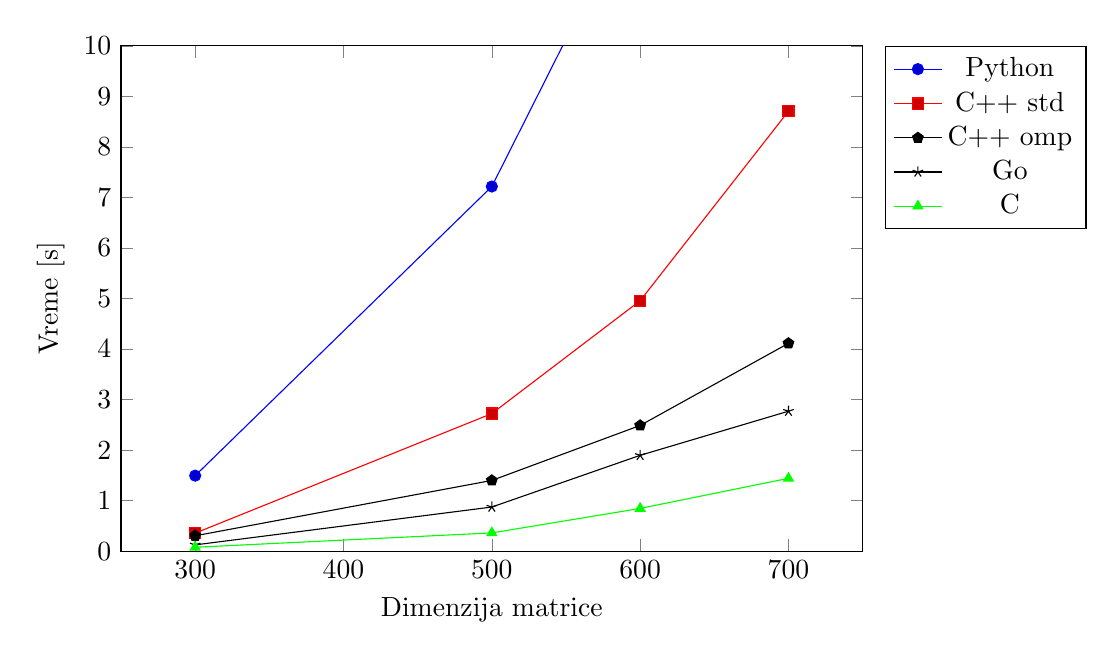
\begin{tikzpicture}
\begin{axis}[
    xlabel={Dimenzija matrice},
    ylabel={Vreme [s]},
    xmin=250, xmax=750,
    ymin=0, ymax=10,
    xtick={300,400,500,600,700},
    ytick={0,1,2,3,4,5,6,7,8,9,10},
    legend pos=outer north east,
    ymajorgrids=true,
    grid=none,
    width=11cm,
    height=8cm,
]
\addplot coordinates {(300,1.495)(500,7.216)(600,13.048)(700,20.756)}; 
\addplot coordinates {(300,0.357)(500,2.723)(600,4.956)(700,8.706)};
\addplot[mark=pentagon*] coordinates {(300,0.305)(500,1.4)(600,2.488)(700,4.113)};
\addplot coordinates {(300,0.125)(500,0.874)(600,1.897)(700,2.77)};
\addplot[green, mark=triangle*] coordinates {(300,0.078)(500,0.362)(600,0.846)(700,1.442)};
\legend{Python,C++ std, C++ omp, Go, C}
\end{axis}
\end{tikzpicture}

\caption{Grafik brzine izvršavanja različitih implementacija množenja matrica u zavisnosti od veličine matrice}
\label{fig:matrix}
\end{center}
\end{figure}

\begin{figure}
\begin{center}

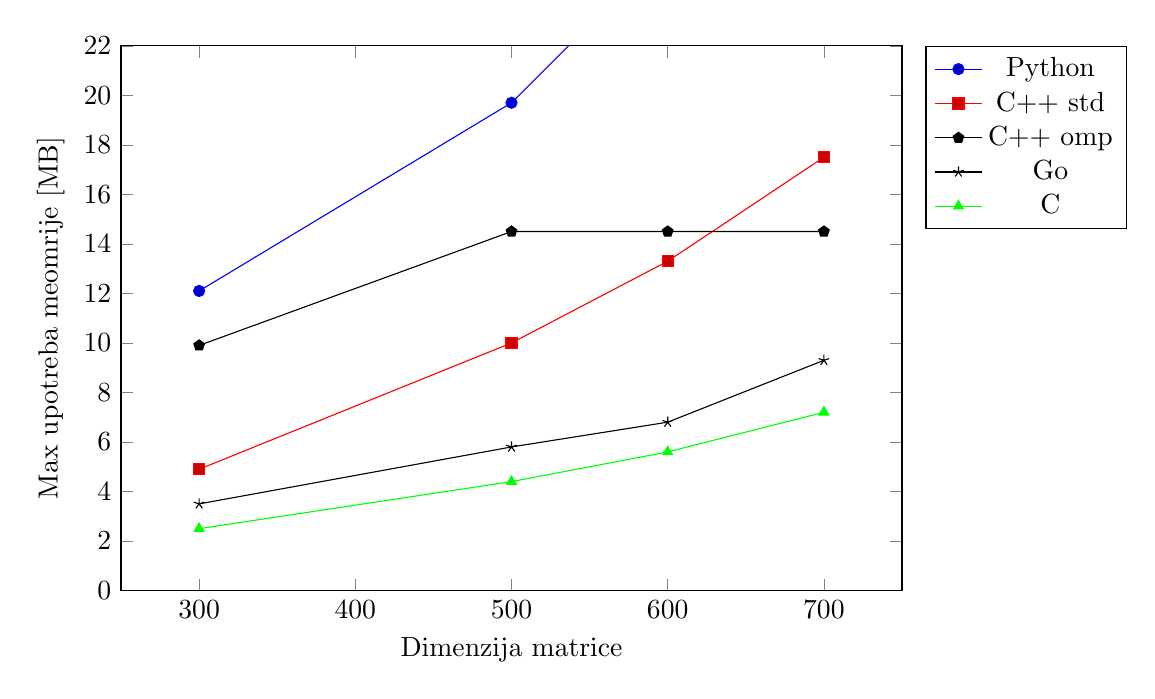
\begin{tikzpicture}
\begin{axis}[
    xlabel={Dimenzija matrice},
    ylabel={Max upotreba meomrije [MB]},
    xmin=250, xmax=750,
    ymin=0, ymax=22,
    xtick={300,400,500,600,700},
    ytick={0,2,4,6,8,10,12,14,16,18,20,22},
    legend pos=outer north east,
    ymajorgrids=true,
    grid=none,
    width=11.5cm,
    height=8.5cm,
]
\addplot coordinates {(300,12.1)(500,19.7)(600,26)}; 
\addplot coordinates {(300,4.9)(500,10)(600,13.3)(700,17.5)};
\addplot[mark=pentagon*] coordinates {(300,9.9)(500,14.5)(600,14.5)(700,14.5)};
\addplot coordinates {(300,3.5)(500,5.8)(600,6.8)(700,9.3)};
\addplot[green, mark=triangle*] coordinates {(300,2.5)(500,4.4)(600,5.6)(700,7.2)};
\legend{Python,C++ std, C++ omp, Go, C}
\end{axis}
\end{tikzpicture}

\caption{Grafik maksimalne upotrebe memorije različitih implementacija množenja matrica u zavisnosti od veličine matrice}
\label{fig:matrix2}
\end{center}
\end{figure}

Broj linija k\^{o}da svih  implementacija je prikazan u tabeli \ref{tab:matrix1}. Najduža implementacija je C++ verzija sa standardnom bibliotekom jer se sastoji iz više fajlova iz razloga što ima razdvojenu konkurentnost od same logike algoritma i kao takva daje više mogućnosti za njeno korišćenje. Python i C++ verzija sa OpenMP bibliotekom imaju najmanji broj linija koda ali se značajno razlikuju. Implementacija u Pythonu je, po mom mišljenju, nepregledna, ne razumljiva i nije intuitivna za korišćenje dok je C++ implementacija uprošćena i krajnje jednostavna. Usled toga što postoji više verzija samog algoritma, na internetu postoji mali broj dostupnih implementacija koje koriste ovu verziju i odgovarajuće biblioteke, ali je i u ovom slučaju dostupan veći broj implementacija za C i C++ nego što je za Python.
 
\begin{table}
\begin{center}
\caption{Dužine k\^{o}da implementacija množenja matrica}
\begin{tabular}{|c|c|c|c|c|c|}
\hline
		& C++ std	&  C 	& Go	& C++ omp	& Python	\\ \hline
Br. linija koda&170		& 90	& 71	&45		&45		\\ \hline
\end{tabular}
\label{tab:matrix1}
\end{center}
\end{table}

% Prime==============================================================================

\section{Eratostenovo sito}
Opis algoritma

\subsection{Go}

Konkurentnost algoritma je ostvarena  pomoću go-rutina radnika. Koristi se globalni niz od n bulovskih promenljivih postavljenih na podrzumevanu vrednost - false umesto na true radi jednostavnosti, a kao posledica, pozicije brojeva koji nisu prosti se postavljaju na true za razliku od originalnog algoritma. Svaka go-rutina dobija svoj opseg u okviru kojeg označava brojeve koji nisu prosti. Funkcija koja kreira go-rutine je prikazana u listingu \ref{lst:prime1}. Za svaki broj koji je trenutno označen kao prost, najpre je potrebno je odrediti njegov prvi umnožak, a zatim, označiti sve njegove umnoške unutar opsega, što je i prikazano u listingu \ref{lst:prime2}. Iako svako go-rutina ima svoj opseg, ona mora da pristrupa i članovima niza drugih go-rutina jer su joj potrebni svi prosti brojevi manji od korena iz n. To kao posledecu dovodi do mogućnost da se u nekim slučajevima bespotrebno eliminišu umnošci brojeva koji nisu prosti, što narušava efikasnost. Problem je rešen tako što se u svakoj iteraciji proverava dodatni uslov: da li je vredost niza, za broj kojem se trenutno eliminišu umnošci, postavljena na true, odnosno, da li je neka druga go-rutina označila da taj broj nije prost. U ovom rešenju dolazi do "data race"-a, međutim, u ovom slučaju je to dopustivo i nisu potrebni muteksi upravo zato što proveravamo dodatni uslov da li je pročitana vrednost u međuvremenu bila menjana. Ako se "data race"  detektor pozove, dobija se izveštaj koji upozorava da postoji "data race". Primer izveštaja se može videti na slici \ref{fig:datarace}. 

\begin{center}
\begin{lstlisting}[caption=Go implementacija konkurentne funkcije za određivanje prostih brojeva manjih od n,label={lst:prime1},float, backgroundcolor=\color{background}]
func Prime(list *[]bool, n int, is_concurrent bool){
	sqrt := int(math.Sqrt(float64(n)))
	first := 0
	step := int(n/ num_goroutines)
	last := step
	wg := sync.WaitGroup{}
	wg.Add(num_goroutines)

	for i:=0; i < num_goroutines-1; i++{
		go mark_prime(list,first,last,sqrt,&wg,true)
		first = last + 1
		last += step
	}

	mark_prime(list,first,n-1,sqrt,&wg)
	wg.Wait()
}
\end{lstlisting}
\end{center}

\begin{center}
\begin{lstlisting}[caption=Go implementacija konkurentne funkcije za označavanje prostih brojeva,label={lst:prime2},float, backgroundcolor=\color{background}]
func mark_prime(list *[]bool,first,last,sqrt int,wg *sync.WaitGroup){
	for i:=2;  i<= sqrt && i*i<= last; i++{
		if !(*list)[i] {
			var j int
			if i*i < first {
				if (first - i*i)%i == 0 {
					j = i*i + ((first-i*i)/i)*i
				}else {
					j = i*i + ((first-i*i)/i + 1)*i
				}
			}else {
				j = i*i
			}
		
			for ; j <= last && !(*list)[i]; j+=i {
				(*list)[j] = true
			}
		}
	}
	wg.Done()
}
\end{lstlisting}
\end{center}

\subsection{C}
Algoritam je implementiran\footnote{\url{https://stackoverflow.com/questions/37407048/sieve-of-eratosthenes-pthread-implementation-thread-number-doesnt-affect-compu}} tako što svaka nit obrađuje tekući prost broj u svom delu opsega. Kada su sve niti završile sa označavanjem tekućeg prostog broja prelazi se na sledeći. Čekanje je realizovano pomoću muteksa koji štiti promenljivu koja označava broj aktivnih niti i broadcast signala koji deblokira sve niti koje čekaju.

\subsection{C++}
U ovoj implementaciji\footnote{\url{http://create.stephan-brumme.com/eratosthenes/}}, koristi se OpenMP biblioteka. Sama implementacija nudi više verzija algoritma i mogućnost da se izvršava konkurentno ili sekvencijalno. Za testiranje je uzeta verzija sa blokovskom raspodelom opsega na sličan način kao što je urađeno u Go implementaciji sa dodatkom da se obrađuju samo neparni brojevi. Obrađivanje svakog bloka se poziva u paralelnoj for petlji.

\subsection{Python}
Implementacija\footnote{\url{http://cs.curs.pub.ro/wiki/asc/_media/asc:lab2:parprocbook.pdf\#page=75}} koristi threading paket za razliku od drugih implementacija u Pythonu koje su do sada pomenute. Prost broj za koji se trenutno elimišu njegovi umnošci je zaštićen katnacem, tako da svaka nit kada dobije katanac čita tekuću vrednost, ažurira je a zatim oslobođa katanac i obrađuje tekuću vrednost nakon čega se proces ponavlja. 

\subsection{Rezultati}
Testiranjem implementacija za različite brojeve n, dobijeni su sledeći rezultati. Vremenska efikasnost implementacija je prikazana u tabeli \ref{tab:prime1}. C++ se pokazao kao najefikasniji i potrebno mu je najmanje vremena za izvršavanje programa. Go implementacija je takođe efikasna ali ipak nešto sporija od C++-a. Python se ponovo najsporije izvršava, ovoga puta toliko da nije bilo mogućnosti testirati ga na ulazima iste veličine. U odnosu na sekvencijalno izvršavanje, Go i C nemaju značajno ubrzanje dok C++ dobija višestruko, ali se ipak Go implementacija pokazala kao najbrža u sekvencijanom režimu rada. Kod Pythona se sekvencijalno izvršavanje pokazalo kao trostuko efikasnije kao posledica loše implementacije. Kada n uzima vrednost milion ili manje, u svim jezicima konkurentno izvršavanje ima istu ili lošiju efikasnost u odnosu na sekvencijalno. To pokazuje da bi konkurentnost trebalo koristiti samo za probleme određene kompleksnosti i veličine a ne kao univerzalno sredstvo za podizanje efikasnosti jer dolazi sa svojom cenom.

\begin{table}
\begin{center}
\caption{Vreme izvršavanja [s] implementacija Eratostenovog sita za različito n}
\begin{tabular}{||c||c|c|c|c||c|c|c|c||}
\hline
&\multicolumn{4}{c||}{Konkurentno izvršavanje}&\multicolumn{4}{c||}{Sekvencijalno izvršavanje} \\ \hline
\diagbox[width=2.7cm, height=1cm]{Jezik}{\vspace*{-0.8cm}n [$10^{6}$]} &1 &100 &300 &500 &1 &100 &300 &500 \\ \hline
C++	& 0,010  		&\textbf{ 0,263}	&\textbf{ 0,770}	&\textbf{1,309}	& 0,008 		&  0,663  		& 2,103		&3,507		\\ 
Go	& \textbf{0,006}	& 0,279		& 0,922		&1,551		&\textbf{ 0,007} 	& \textbf{ 0,349}  	& \textbf{1,178}	&\textbf{2,110}	\\
C 	& 0,025		& 2,178  		& 7,007		&12,416		& 0,016 		&  2,529		& 8,245		&14,524		\\ \hline
\diagbox[width=2.7cm, height=1cm]{Jezik}{\vspace*{-0.8cm}n [$10^{6}$]}& 0,1	&1	&10	&30 & 0,1	&1	&10	&30\\ \hline
Python& 0,107		& 1,185	& 13,702	&39,321	& 0,071	&  0,378	& 4,214	&13,487 	\\ \hline
\end{tabular}
\label{tab:prime1}
\end{center}
\end{table}

Maksimalna upotreba memorije se može videti u tabeli \ref{tab:prime2}. Implementacija u C++-u nije prikazana jer ne čuva listu svih prostih brojeva i kao rezultat ima konstantnu upotrebu memorije od 3MB. Go i C imaju približno iste memorijske zahteve ali se C pokazao kao efikasniji, dok je Python ponovo najzahtevniji. Za sekvencijalno izvršavanje Go i C koriste istu količinu memorije kao i za konkurentno. Python-u je potrebno 50\% više memorije pri konkuretnom izvršavanju nego sekvencijalnom. 

\begin{table}
\begin{center}
\caption{Maksimalna upotreba memorije [MB] implementacija Eratostenovog sita za različito n}
\begin{tabular}{|c|c|c|c|c|}
\hline
\diagbox[width=2.7cm, height=1cm]{Jezik}{\vspace*{-0.8cm}n [$10^{6}$]} &1 &100 &300 &500 \\ \hline
C  	 & 2,0		& 98,8	&293,9	&489,6	 \\ \hline
Go  	 & 4,0		& 107,2	&315,6	&523,7	 \\ \hline
\diagbox[width=2.7cm, height=1cm]{Jezik}{\vspace*{-0.8cm}n [$10^{6}$]}& 0,1	&1	&10	&30\\ \hline
Python& 13,7	& 29,7	&123,1	&677,2	 \\ \hline
\end{tabular}
\label{tab:prime2}
\end{center}
\end{table}

Go implementacija je testirana za različite vrednosti promenljive koja označava broj go-rutina i rezultati se mogu pogledati u tabeli \ref{tab:prime3}. Svi do sada prikazani rezultati su testirani sa 1000 go-rutina. Ako se smanji broj go-rutina na 100 vremenska efikasnost drastično opada, međutim ako se poveća na 10000, vremenska efikasnost ostaje ista ali je potrebno 20MB više. Gledajući rezultate vidimo da promenljiva ima uticaj i na sekvencijalno izvršavanje iz razloga što ona ima ulogu određivanja veličine bloka koji će svaka funkcija obrađivati. Kod ove implementacije je neophodno odrediti minimalan broj go-rutina za koji se postiže maskimalna vremenska efikasnost, što je u ovom sličaju eksperimentalno utvrđeno da je 1000. 

\begin{table}
\begin{center}
\caption{Performanse Go implementacije za različite vrednosti promenljive koja označava broj go-rutina kada je n= $500*10^{6}$}
\begin{tabular}{||c||c|c||c|c||}
\hline
&\multicolumn{2}{c||}{Konkurentno izvršavanje}&\multicolumn{2}{c||}{Sekvencijalno izvršavanje} \\ \hline
Br. go-rutina	& Vreme [s]& Memorija [kB]& Vreme [s]& Memorija [kB]\\ \hline
100		& 11,996	& 520.296	&7,158	&520.048\\ \hline
1000		& 1,551	& 523.684	&2,110 	&520.088\\ \hline
10000		& 1,568	& 544.996	&2.190	&521456\\ \hline
\end{tabular}
\label{tab:prime3}
\end{center}
\end{table}

Dužine implementacija su prikazane u tabeli \ref{tab:prime4}. Najduža implementacija je u C-u, dok je u Pythonu ponovo najkraća. C++ implementacija je, po mom mišljenju, najkvalitetnija jer nudi više verzija samog algoritma i pokazala se kao najefikasnija. Za ovaj algoritam nije dostupan veliki broj konkurentnih implementacija ali je moguće pronaći efikasne za C i C++, dok je za Python dostupna implementacija koja je iskorišćena, napravljena za ilustrativne svrhe i neefikasna.

\begin{table}
\begin{center}
\caption{Dužine k\^{o}da implementacija Eratostenovog sita}
\begin{tabular}{|c|c|c|c|c|}
\hline
		&  C  		&C++ 	& Go 	& Python 	 \\ \hline
Br. linija koda& 151		& 100		&75	&45		 \\ \hline
\end{tabular}
\label{tab:prime4}
\end{center}
\end{table}


\section{Složeniji primeri u programskom jeziku Go}




\chapter{Zaključak}





\printbibliography 
% ==============================================================================
% Završni deo teze i prilozi
\backmatter
% ==============================================================================



\end{document}
